% 文件路径: content/02_RandomProcesses/run_chapter02.tex

% 1. 调用根目录 cls (../../ 指向项目根目录)
\documentclass{../../commsummary}

% 2. 修正图片路径
\graphicspath{{./figures/}{../../figures/}}

\begin{document}

% 3. 临时标题 (Dev Mode)
\section{随机过程 (独立编译)}

% 4. 导入本章 Topic
% (顺序已与 main.tex 保持一致)

% 基础定义与平稳性
\begin{kbox}{1. 随机过程定义与统计特性}
    \textbf{定义}:
    随时间作随机变化的一系列随机变量的集合。
        \begin{itemize}[leftmargin=3em]
            \item[(1)] 结构上是:所有样本函数 $\xi_i(t)$ 的集合;
            \item[(2)] 也是随机变量 $\xi(t)$ 的集合。
        \end{itemize}

    \tcbline

    \textbf{统计特性与物理意义}:
    \begin{itemize}
        \item \textbf{一维分布函数}:
        \[ F_1(x_1, t_1) = P\{\xi(t_1) \leq x_1\} \]
        \item \textbf{一维概率密度函数 (PDF)}:
        \[ f_1(x_1, t_1) = \frac{\partial F_1(x_1, t_1)}{\partial x_1} \]
        \item \textbf{均值 (数学期望)} —— \textcolor{mainblue}{直流分量}:
        \[ \mu(t) = E[\xi(t)] = \int_{-\infty}^{\infty} x f_1(x, t) dx \]
        \item \textbf{方差} —— \textcolor{mainblue}{交流功率}:
        \[ \sigma^2(t) = D[\xi(t)] = E\left[(\xi(t) - \mu(t))^2\right] \]
        \item \textbf{平均功率 (二阶原点矩)}:
        由 $DX = E(X^2) - (EX)^2$ 可知功率关系:
        \[ \underbrace{E[\xi^2(t)]}_{\text{平均功率}} = \underbrace{\sigma^2(t)}_{\text{交流功率}} + \underbrace{\mu^2(t)}_{\text{直流功率}} \]
        (当 $\mu(t)=0$ 时,平均功率等于交流功率)
        
        \item \textbf{自相关函数}:
        描述同一过程在任意两个时刻随机变量间的关联程度。
        \begin{align*}
            R(t_1, t_2) &= E[\xi(t_1)\xi(t_2)] \\
            &= \iint_{-\infty}^{\infty} x_1 x_2 f_2(x_1, x_2; t_1, t_2) dx_1 dx_2
        \end{align*}
        (其中 $f_2$ 为二维概率密度函数)
        
        \item \textbf{互相关函数}:
        \[ R_{\xi\eta}(t_1, t_2) = E[\xi(t_1)\eta(t_2)] \]
    \end{itemize}
\end{kbox}

% --- 核心概念辨析 ---
\begin{kbox}{核心概念辨析:样本函数 vs 随机变量}
    \textbf{误区}:随机过程的“样本”不是随机变量,二者观察维度不同。
    
    对于随机过程 $\xi(t, \omega)$:
    \begin{itemize}
        \item \textbf{样本函数 (Sample Function)}:\textcolor{alertred}{固定 $\omega$,变化 $t$}。
        \\ 指随机过程的\textbf{一次具体实现}(如做了一次实验记录下的波形)。既然实验已发生,它就是一条\textbf{确定的时间函数} $x(t)$,不再具有随机性。
        \item \textbf{随机变量 (Random Variable)}:\textcolor{alertred}{固定 $t$,变化 $\omega$}。
        \\ 指随机过程在\textbf{某一特定时刻}的状态。它包含该时刻所有可能的取值及其概率分布,是\textbf{随机的}。
        \item \textbf{总结}:样本函数是“时间的函数”,随机变量是“概率的函数”。二者同时固定时,唯一确定一个数值。
    \end{itemize}
    
    \tcbline
    
    \textbf{直观总结}:
    \begin{itemize}
        \item “样本”是\textbf{纵向的历史轨迹}(确定的曲线)。
        \item “随机变量”是\textbf{横向的时间切片}(统计分布)。
    \end{itemize}
\end{kbox}
\begin{kbox}{2. 平稳随机过程}
    \textbf{广义平稳 (WSS) 条件}:
    \begin{enumerate}
        \item 均值与时间无关:$\mu(t) = \mu$
        \item 自相关仅与间隔 $\tau$ 有关:$R(t_1, t_1 + \tau) = R(\tau)$
    \end{enumerate}

    \tcbline

    \textbf{狭义平稳 (SSS) 与 广义平稳 (WSS) 对比}:
    \begin{itemize}
        \item \textbf{定义区别}:SSS 要求所有统计特性不变;WSS 仅要求均值和自相关不变。
        \item \textbf{关系}:SSS (二阶矩有限) $\Rightarrow$ WSS;反之通常不成立
        \item \textbf{特例}:对于\textbf{高斯随机过程},WSS $\Leftrightarrow$ SSS。
    \end{itemize}
    
    \tcbline 
    
    \textbf{各态历经性 (遍历性)}:
    \begin{itemize}
        \item \textbf{定义}:若平稳过程的\textbf{统计平均}等于样本的\textbf{时间平均},则称其具有各态历经性。
        \item \textbf{意义}:\textbf{用一次实现的时间平均取代过程的统计平均}。简化测量,因为实际往往只有一个样本波形。
        \item \textbf{数学条件}:$\mu = \bar{\mu}$ 且 $R(\tau) = \bar{R}(\tau)$。
    \end{itemize}
    
    \tcbline
    
    \textbf{深入理解:各态历经性与平稳性的关系}
    \begin{itemize}
        \item \textbf{为什么任一样本能代表整体?} \\
        各态历经的物理含义是:\textbf{一个样本在无限长的时间内,遍历了随机过程所有可能的状态}。因此,观测这一个样本足够久,就等同于观测了整个集合。
        
        \item \textbf{为什么“各态历经 $\Rightarrow$ 平稳”?} \\
        因为“时间平均”是一个常数(积分区间是无穷大),若它等于“统计平均”,则统计平均也必须是常数(不随 $t$ 变化),这正是平稳过程的定义。
        
        \item \textbf{为什么“平稳 $\nRightarrow$ 各态历经”?} \\
        平稳只要求整体统计特性不变,但允许样本之间存在永久性差异(“老死不相往来”)。
        \\ \textit{反例}:$X(t)=C$($C$为随机常数)。样本要么恒为1,要么恒为-1。单个样本的时间平均(1或-1)不等于整体统计平均(0),它没有遍历所有状态。
    \end{itemize}
\end{kbox}

% 自相关与功率谱
\begin{kbox}{3. 自相关函数与功率谱密度}
    \textbf{自相关函数 $R(\tau)= E[\xi(t)\xi(t+\tau)]$ 的性质}:
    \begin{enumerate}
        \item 偶函数:$R(\tau) = R(-\tau)$
        \item 最大值:$|R(\tau)| \leq R(0)$
        \item 平均功率:$R(0) = E[\xi^2(t)]$
        \item 直流功率:$R(\infty) = E^2[\xi(t)] = \mu^2$
        \item 交流功率 (方差):$\sigma^2 = R(0) - R(\infty)$
    \end{enumerate}
    
    \vspace{4pt}
    \noindent\tikz\draw[dashed, mainblue!50] (0,0) -- (\linewidth,0);
    \vspace{4pt}
    
    \textbf{\small \textcolor{gray}{性质证明简述 (Proof Sketch)}}
    \small
    \begin{itemize}
        \item \textbf{偶函数}:令 $t' = t-\tau$ 换元,则 $E[\xi(t)\xi(t-\tau)] \Rightarrow E[\xi(t'+\tau)\xi(t')] = R(\tau)$。
        \item \textbf{最大值}:由柯西-施瓦茨不等式 $|E[XY]|^2 \leq E[X^2]E[Y^2]$,令 $X=\xi(t), Y=\xi(t+\tau)$,因平稳性 $E[X^2]=E[Y^2]=R(0)$,得证。
        \item \textbf{直流功率}:当 $\tau \to \infty$,$\xi(t)$ 与 $\xi(t+\tau)$ 去相关 (独立),期望可拆分:$E[\xi(t)\xi(t+\tau)] \approx E[\xi(t)]E[\xi(t+\tau)] = \mu^2$。
        \item \textbf{交流功率}:由方差定义 $\sigma^2 = E[\xi^2] - (E[\xi])^2$,代入即得 $R(0) - R(\infty)$。
    \end{itemize}
    \normalsize
    
    \tcbline
    
    \textbf{维纳-辛钦定理 (PSD)}:
    平稳过程的功率谱密度 $P_{\xi}(\omega)$ 与 $R(\tau)$ 互为傅里叶变换对:
    \begin{align*}
        P_{\xi}(\omega) &= \int_{-\infty}^{\infty} R(\tau) e^{-j\omega\tau} d\tau \\
        R(\tau) &= \int_{-\infty}^{\infty}  P_{\xi}(f) e^{j2\pi f \tau} df
    \end{align*}
\end{kbox}

\begin{kbox}{核心概念辨析:自相关函数值的物理意义}
    \textbf{1. 为什么 $R(0)$ 是总平均功率?}
    \begin{itemize}
        \item \textbf{数学定义}:$R(0) = E[X(t)X(t)] = E[X^2(t)]$,即均方值。
        \item \textbf{物理直观}:$\tau=0$ 时,信号与其自身完全重合,\textbf{相关性最强}。此时记录的是信号在任一时刻的总能量,包含了\textbf{恒定的直流分量}和\textbf{起伏的交流分量}。
    \end{itemize}

    \tcbline

    \textbf{2. 为什么 $R(\infty)$ 是直流功率?}
    \begin{itemize}
        \item \textbf{去相关性 (Decorrelation)}:
        对于非周期的平稳过程,随着时间间隔 $\tau$ 的增大,随机起伏(交流)部分的信号会逐渐失去联系(失去“记忆”)。
        \item \textbf{数学推导}:
        当 $\tau \to \infty$ 时,$X(t)$ 与 $X(t+\tau)$ 变得\textbf{互不相关}。
        \[ \lim_{\tau \to \infty} E[X(t)X(t+\tau)] = E[X(t)] \cdot E[X(t+\tau)]  = \mu^2 \]
        \item \textbf{物理含义}:
        时间拉得足够长后,交流波动的相关性衰减为 0,唯有\textbf{永恒不变的直流分量}依然保持完全相关。因此,剩下的“残留”相关值就是直流功率。
    \end{itemize}

    \tcbline
    
    \textbf{3. 总结}
    \[ \underbrace{R(0)}_{\text{总功率}} = \underbrace{R(\infty)}_{\text{直流功率}} + \underbrace{\sigma^2}_{\text{交流功率 (方差)}} \]
\end{kbox}


% --- 新增部分:平稳性与变换的深入辨析 ---
\begin{kbox}{深入辨析:维纳-辛钦定理的适用细节}
    \textbf{1. 为什么必须是平稳过程?}
    \begin{itemize}
        \item \textbf{定理限制}:$P_{\xi}(\omega) = \mathcal{F}\{R(\tau)\}$ 仅对\textbf{宽平稳 (WSS)} 过程严格成立。
        \item \textbf{非平稳情况}:若 $X(t)$ 非平稳,自相关 $R(t_1, t_2)$ 随绝对时间变化,无法定义单一的“静态”功率谱。
        \item \textbf{工程处理}:通常采用\textbf{时间平均自相关}(求平均功率谱)或\textbf{时频分析}(如 Wigner-Ville 分布)来描述随时间变化的频谱。
    \end{itemize}

    \tcbline

    \textbf{2. 傅里叶逆变换:$\omega$ 与 $f$ 的系数之谜}
    \begin{itemize}
        \item \textbf{角频率 $\omega$ (需系数 $\frac{1}{2\pi}$)}:
        \[ R(\tau) = \frac{1}{2\pi} \int_{-\infty}^{\infty} P_{\xi}(\omega) e^{j\omega\tau} d\omega \]
        这里的 $\frac{1}{2\pi}$ 用于抵消 $d\omega$ 带来的 $2\pi$ 倍积分增益。
        \item \textbf{频率 $f$ (系数为 1)}:
        \[ R(\tau) = \int_{-\infty}^{\infty} P_{\xi}(f) e^{j2\pi f \tau} df \]
        \item \textbf{物理一致性}:工程记号 $P_{\xi}(f)$ 实际上等价于数学上的 $P_{\xi}(2\pi f)$。即在同一物理频率点(例如 10Hz 与 $20\pi$ rad/s),其功率密度值是相等的。
    \end{itemize}
\end{kbox}

% 高斯过程与线性系统
\begin{kbox}{4. 高斯随机过程与误差函数 (基础结论)}
    \textbf{1. 概率密度与分布函数}
    \begin{itemize}
        \item \textbf{概率密度 (PDF)}:
        \[ f(x) = \frac{1}{\sqrt{2\pi}\sigma} \exp\left[-\frac{(x-\mu)^2}{2\sigma^2}\right] \]
        \item \textbf{分布函数 (CDF) 定义}:
        分布函数是 PDF 的积分(即 $x$ 落在 $(-\infty, b]$ 的概率):
        \[ F(b) = P(x \leq b) = \int_{-\infty}^{b} \frac{1}{\sqrt{2\pi}\sigma} \exp\left[-\frac{(x-\mu)^2}{2\sigma^2}\right] dx \]
    \end{itemize}
    
    \tcbline
    
    \textbf{2. 误差函数的由来}
    上述积分无法用初等函数直接表示,引入定义:
    \[ \mathrm{erf}(z) \triangleq \frac{2}{\sqrt{\pi}} \int_0^z e^{-u^2} du \]
    {\small \textcolor{gray}{注:系数 $2/\sqrt{\pi}$ 是为了归一化,确保 $\mathrm{erf}(\infty)=1$。}}
    
    \tcbline
    
    \textbf{3. $F(x)$ 的分段表达式}
    \[
    F(x) = 
    \begin{cases}
        \displaystyle \frac{1}{2} + \frac{1}{2} \mathrm{erf}\left( \frac{x-\mu}{\sqrt{2}\sigma} \right), & x \geq \mu \\[1.2em]
        \displaystyle 1 - \frac{1}{2} \mathrm{erfc}\left( \frac{x-\mu}{\sqrt{2}\sigma} \right), & x < \mu
    \end{cases}
    \]
\end{kbox}

% --- 插入详细推导部分 ---
\begin{kbox}{补充推导:高斯分布与误差函数详解}
    \textbf{1. 高斯随机过程定义} \\
    随机变量 $\xi(t)$ 的任意 $n$ 维分布服从正态分布,称为高斯过程。

    \tcbline

    % --- 新增部分:来自图片内容 ---
    \textbf{2. 高斯过程的重要性质}
    \begin{itemize}
        \item 高斯过程的 $n$ 维概率密度函数仅取决于它的\textcolor{red}{数学期望}、\textcolor{red}{方差}和\textcolor{red}{相关函数}。
        \item 对高斯过程,\textcolor{red}{广义平稳} $\Leftrightarrow$ \textcolor{red}{严平稳}。
        \item 高斯过程,在不同时刻的随机变量值,\textcolor{red}{互不相关} $\Leftrightarrow$ \textcolor{red}{互相独立}。
        \item 高斯过程(变量)的\textcolor{red}{线性变换}仍为高斯过程(变量)。
    \end{itemize}

    \tcbline
    % ---------------------------

    \textbf{3. 互补误差函数性质}
    \begin{align*}
        \text{erfc}(-z) &= 1 - \text{erf}(-z) \\
        &= 1 + \text{erf}(z) \\
        &= 2 - \text{erfc}(z)
    \end{align*}
    即:\textcolor{mainblue}{$\text{erfc}(z) + \text{erfc}(-z) = 2$}

    \tcbline

    \textbf{4. 分布函数 $F(x)$ 的积分推导细节} \\
    设正态分布概率密度函数为 $f(t)$,则分布函数 $F(x) = \int_{-\infty}^{x} f(t) dt$。

    \vspace{4pt}
    \textbf{(1) 当 $x > \mu$ 时 (落在均值右侧)}
    \[ F(x) = \int_{-\infty}^{\mu} f(t) dt + \int_{\mu}^{x} \frac{1}{\sqrt{2\pi}\sigma} e^{-\frac{(t-\mu)^2}{2\sigma^2}} dt \]
    显然由高斯分布对称性知:$\int_{-\infty}^{\mu} f(t) dt = \frac{1}{2}$。
    
    \textbf{换元法}:对后式,令 $y = \frac{t-\mu}{\sqrt{2}\sigma}$,则 $dy = \frac{1}{\sqrt{2}\sigma} dt$。
    \begin{itemize}
        \item 当 $t=x$ 时,$y=\frac{x-\mu}{\sqrt{2}\sigma}$;
        \item 当 $t=\mu$ 时,$y=0$。
    \end{itemize}
    代入积分项:
    \[ \int_{\mu}^{x} f(t) dt = \int_{0}^{\frac{x-\mu}{\sqrt{2}\sigma}} \frac{1}{\sqrt{\pi}} e^{-y^2} dy \]
    根据 $\text{erf}(z) = \frac{2}{\sqrt{\pi}} \int_{0}^{z} e^{-u^2} du$ 的定义,上式即为 $\frac{1}{2}\text{erf}(\frac{x-\mu}{\sqrt{2}\sigma})$。
    
    \noindent \textbf{故当 $x > \mu$ 时:}
    \[ \boxed{F(x) = \frac{1}{2} + \frac{1}{2} \text{erf}\left(\frac{x-\mu}{\sqrt{2}\sigma}\right)} \]

    \vspace{4pt}
    \textbf{(2) 当 $x < \mu$ 时 (落在均值左侧)}
    \[ F(x) = \int_{-\infty}^{\mu} f(t) dt - \int_{x}^{\mu} \frac{1}{\sqrt{2\pi}\sigma} e^{-\frac{(t-\mu)^2}{2\sigma^2}} dt \]
    同样利用对称性 $\int_{-\infty}^{\mu} f(t) dt = \frac{1}{2}$。
    
    \textbf{换元法}:对后式,令 $y = \frac{\mu-t}{\sqrt{2}\sigma}$,则 $dt = -\sqrt{2}\sigma dy$。
    \begin{itemize}
        \item 当 $t=x$ 时,$y=\frac{\mu-x}{\sqrt{2}\sigma}$;
        \item 当 $t=\mu$ 时,$y=0$。
    \end{itemize}
    (注意积分限变换抵消了负号),代入有:
    \[ \int_{x}^{\mu} f(t) dt = \int_{0}^{\frac{\mu-x}{\sqrt{2}\sigma}} \frac{1}{\sqrt{\pi}} e^{-y^2} dy = \frac{1}{2}\text{erf}\left(\frac{\mu-x}{\sqrt{2}\sigma}\right) \]
    
    \noindent \textbf{故当 $x < \mu$ 时:}
    \[ F(x) = \frac{1}{2} - \frac{1}{2} \text{erf}\left(\frac{\mu-x}{\sqrt{2}\sigma}\right) \]

    \tcbline

    \textbf{5. 统一用 $\text{erfc}$ 表示}
    
    又 $\text{erf}(x) = 1 - \text{erfc}(x)$,且 $\text{erfc}(-x) = 2 - \text{erfc}(x)$。
    
    对于 $x < \mu$ 的情况,直接代入:
    \[ 
    \begin{aligned}
        F(x) &= \frac{1}{2} \left[1 - \text{erf}\left(\frac{\mu-x}{\sqrt{2}\sigma}\right)\right] \\
             &= \textcolor{mainblue}{\frac{1}{2} \text{erfc}\left(\frac{\mu-x}{\sqrt{2}\sigma}\right)} 
    \end{aligned}
    \]
    
    对于 $x > \mu$ 的情况:
    \[ 
    \begin{aligned}
        F(x) &= \frac{1}{2} \left[2 - \text{erfc}\left(\frac{x-\mu}{\sqrt{2}\sigma}\right)\right] \\
             &= \textcolor{mainblue}{1 - \frac{1}{2} \text{erfc}\left(\frac{x-\mu}{\sqrt{2}\sigma}\right)} 
    \end{aligned}
    \]
\end{kbox}
% --- 上半部分:核心结论速查 (蓝色盒子) ---
\begin{kbox}{5. 随机过程通过线性系统 (核心结论)}
    \textbf{1. 系统定义}
    \[ \xi_o(t) = \int_{-\infty}^{+\infty} h(\tau)\xi_i(t-\tau) d\tau \]
    
    \tcbline

    \textbf{2. 统计特性三要素}
    \begin{itemize}
        \item \textbf{均值 (直流)}: 
        \[ E[\xi_o(t)] = E[\xi_i(t)] \cdot H(0) \]
        \item \textbf{自相关函数}: 
        \[ R_o(\tau) = R_i(\tau) * h(\tau) * h(-\tau) \]
        \item \textbf{功率谱密度 (重点)}: 
        \[ P_o(f) = |H(f)|^2 P_i(f) \]
        其中 $|H(f)|^2$ 为功率增益。
    \end{itemize}
\end{kbox}

% --- 下半部分:详细推导笔记 (红色盒子) ---
\begin{examplebox}{笔记详解:推导与证明过程}
    \textbf{1. 均值 (期望) 推导}
    \begin{align*}
        E[\xi_o(t)] &= E\left[ \int_{-\infty}^{+\infty} h(\tau)\xi_i(t-\tau) d\tau \right] \\
        &= \int_{-\infty}^{+\infty} h(\tau) \underbrace{E[\xi_i(t-\tau)]}_{a} d\tau
    \end{align*}
    由于输入为平稳随机过程,$E[\xi_i(t)]=a$。由系统函数定义 $H(\omega)$,令 $\omega=0$:
    \[ \boxed{ E[\xi_o(t)] = a \cdot H(0) } \]

    \tcbline

    \textbf{2. 自相关函数与平稳性证明} \\
    计算输出的自相关函数 $R_o(t_1, t_1+\tau)$:
    \begin{align*}
        & E\left[ \left( \int h(\alpha)\xi_i(t_1-\alpha) d\alpha \right) \left( \int h(\beta)\xi_i(t_1+\tau-\beta) d\beta \right) \right] \\
        &= \iint h(\alpha)h(\beta) R_i(\underbrace{\tau+\alpha-\beta}_{\text{时间差}}) d\alpha d\beta
    \end{align*}
    \textbf{结论:} 积分后结果与 $t_1$ 无关,只与 $\tau$ 有关,故输出 $\xi_o(t)$ 仍为\textbf{广义平稳}。

    \tcbline

    \textbf{3. 功率谱密度 (维纳—辛钦定理)} \\
    由 $P_o(f) = \int_{-\infty}^{+\infty} R_o(\tau) e^{-j\omega\tau} d\tau$,代入上式并换元(令 $\tau' = \tau + \alpha - \beta$)。
    
    \vspace{4pt}
    \textit{注:由于公式较长,此处分行显示:}
    \begin{align*}
        P_o(f) &= \iiint h(\alpha)h(\beta) R_i(\tau') \\
               &\quad \cdot e^{-j\omega(\tau'-\alpha+\beta)} \, d\alpha d\beta d\tau'
    \end{align*}

    \textbf{分离变量:}
    \begin{align*}
        = \quad & \underbrace{\int h(\alpha)e^{j\omega\alpha} d\alpha}_{H^*(f)} \\
        \cdot \quad & \underbrace{\int h(\beta)e^{-j\omega\beta} d\beta}_{H(f)} \\
        \cdot \quad & \underbrace{\int R_i(\tau')e^{-j\omega\tau'} d\tau'}_{P_i(f)}
    \end{align*}

    \textbf{最终结果:}
    \[ \boxed{ P_o(f) = |H(f)|^2 P_i(f) } \]
\end{examplebox}

% --- 窄带随机过程与噪声 (核心难点) ---
\begin{kbox}{6. 窄带随机过程 (核心结论)}
    \textbf{定义}:带宽 $\Delta f \ll f_c$ 且远离零频的随机过程。
    
    \tcbline
    
    \begin{minipage}{0.65\linewidth}
        \textbf{表达式}:
        \begin{itemize}
            \item \textbf{包络相位法}:
            \[ \xi(t) = a_{\xi}(t) \cos[\omega_c t + \phi_{\xi}(t)] \]
            \item \textbf{同相正交法}:
            \[ \xi(t) = \xi_c(t) \cos \omega_c t - \xi_s(t) \sin \omega_c t \]
        \end{itemize}
    \end{minipage}%
    \begin{minipage}{0.35\linewidth}
        \centering
        % 融入笔记中的矢量三角形
        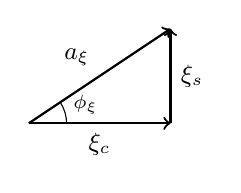
\begin{tikzpicture}[scale=1.2]
            \draw[thick, ->] (0,0) -- (1.5,0) node[midway, below] {\small $\xi_c$};
            \draw[thick, ->] (1.5,0) -- (1.5,1.0) node[midway, right] {\small $\xi_s$};
            \draw[thick, ->] (0,0) -- (1.5,1.0) node[midway, above left] {\small $a_\xi$};
            \draw (0.4,0) arc (0:33.69:0.4);
            \node at (0.6,0.2) {\scriptsize $\phi_\xi$};
        \end{tikzpicture}
    \end{minipage}

    \tcbline 
    
    \textbf{统计特性} (设 $\xi(t)$ 均值0,方差 $\sigma_{\xi}^2$):
    \begin{enumerate}
        \item $\xi_c(t), \xi_s(t)$ 均为高斯过程,均值0,方差 $\sigma_{\xi}^2$。
        \item \textbf{重要结论}:同一时刻,$\xi_c$ 与 $\xi_s$ \textbf{互不相关} (即统计独立)。
        \item \textbf{包络 $a_{\xi}$ (瑞利分布)}:$f(a_{\xi}) = \frac{a_{\xi}}{\sigma_{\xi}^2} e^{-\frac{a_{\xi}^2}{2\sigma_{\xi}^2}}, \ (a_{\xi} \geq 0)$
        \item \textbf{相位 $\phi_{\xi}$ (均匀分布)}:$f(\phi_{\xi}) = \frac{1}{2\pi}, \ (0 \leq \phi_{\xi} \leq 2\pi)$
    \end{enumerate}
\end{kbox}

\begin{kbox}{7. 白噪声与带限噪声}
    \textbf{基本概念}:
    \begin{itemize}
        \item \textbf{白噪声}:在整个频带内功率谱密度 (PSD) 都平坦的噪声。
        \item \textbf{高斯白噪声}:概率分布服从高斯分布,且 PSD 均匀的噪声。
        \item \textbf{带限白噪声}:白噪声通过有限带宽信道或滤波器后的噪声。
    \end{itemize}

    \tcbline

    \textbf{理想白噪声}:
    \begin{itemize}
        \item PSD (双边):$P_n(f) = n_0 / 2$
        \item 自相关:$R(\tau) = \frac{n_0}{2} \delta(\tau)$
    \end{itemize}
    
    \textbf{低通白噪声 (LPF, 截止 $f_H$)}:
    \[ R(\tau) = n_0 f_H \frac{\sin 2\pi f_H \tau}{2\pi f_H \tau} = n_0 f_H \operatorname{Sa}(2\pi f_H \tau) \] 
    
    \textbf{带通白噪声 (BPF, 带宽 $B$)}:
    \[ R(\tau) = n_0 B \frac{\sin \pi B \tau}{\pi B \tau} \cos 2\pi f_c \tau, \quad N = n_0 B \]
\end{kbox}

\begin{kbox}{8. 正弦波 + 窄带高斯噪声}
    \textbf{包络 $z$ 服从莱斯 (Rice) 分布}:
    \[ f(z) = \frac{z}{\sigma_n^2} \exp\left[-\frac{z^2 + A^2}{2\sigma_n^2}\right] I_0\left(\frac{Az}{\sigma_n^2}\right) \]
    ($A$: 信号振幅, $\sigma_n^2$: 噪声方差, $I_0$: 修正贝塞尔)
\end{kbox}
\definecolor{mainblue}{RGB}{20, 80, 180}
\definecolor{fillblue}{RGB}{220, 230, 255}

\begin{examplebox}{补充:窄带过程推导与图解}
    \textbf{1. 正交分解推导细节}:
    利用三角公式展开 $\xi(t) = a_\xi(t) \cos[\omega_c t + \phi_\xi(t)]$:
    \begin{align*}
        \xi(t) &= a_\xi [\cos \phi_\xi \cos \omega_c t - \sin \phi_\xi \sin \omega_c t] \\
               &= \underbrace{[a_\xi \cos \phi_\xi]}_{\xi_c(t)} \cos \omega_c t - \underbrace{[a_\xi \sin \phi_\xi]}_{\xi_s(t)} \sin \omega_c t
    \end{align*}
    转换关系:
    \[ a_\xi = \sqrt{\xi_c^2 + \xi_s^2}, \quad \phi_\xi = \arctan(\xi_s / \xi_c) \]

    \tcbline

    \textbf{2. 概率密度函数图示}:
    \begin{center}
        \begin{tikzpicture}[font=\small]
            % --- 左图:瑞利分布 ---
            \begin{axis}[
                name=plot1,
                width=0.48\textwidth, height=5.5cm,
                axis lines=middle,
                xmin=0, xmax=4.2, ymin=0, ymax=0.75,
                xlabel={$a_\xi$}, ylabel={$f(a_\xi)$},
                ticks=none,
                axis line style={-latex, thick, black!80},
                xlabel style={right}, ylabel style={above},
                title={\textbf{瑞利分布 (包络)}},
                % --- 修改处:向上移动标题 15pt,并稍微加大字号 ---
                title style={yshift=15pt, font=\large}, 
                clip=false
            ]
                % 1. 绘制面积条带
                \fill[fillblue] (axis cs:1.2, 0) rectangle (axis cs:1.35, 0.48);
                
                % 2. 瑞利曲线
                \addplot[thick, mainblue, domain=0:4.0, samples=200] {x*exp(-x^2/2)};
                
                % 3. 均值虚线
                \draw[dashed, thick, black!60] (axis cs:1.253, 0) -- (axis cs:1.253, 0.455);
                
                % 4. 底部坐标标注
                \node[below] at (axis cs:1.253, 0) {$\sqrt{\frac{\pi}{2}}\sigma_\xi$};
                
                % 5. 文本公式
                \node[right, align=left] at (axis cs:1.8, 0.5) {
                    均值 $=\sqrt{\frac{\pi}{2}}\sigma_\xi$ \\[0.5em]
                    方差 $=\frac{4-\pi}{2}\sigma_\xi^2$
                };
                
                % 6. "等面积" 标注
                \node[coordinate, pin={[pin edge={black, thin}, align=center]120:等面积}] at (axis cs:1.27, 0.25) {};
                
            \end{axis}

            % --- 右图:均匀分布 ---
            \begin{axis}[
                at={(plot1.outer east)}, anchor=outer west,
                width=0.48\textwidth, height=5.5cm,
                axis lines=middle,
                xmin=0, xmax=7.5, ymin=0, ymax=0.35,
                xlabel={$\phi_\xi$}, ylabel={$f(\phi_\xi)$},
                ticks=none,
                axis line style={-latex, thick, black!80},
                xlabel style={right}, ylabel style={above},
                title={\textbf{均匀分布 (相位)}},
                % --- 修改处:同样向上移动标题 15pt ---
                title style={yshift=15pt, font=\large},
                clip=false
            ]
                % 1. 均匀分布矩形
                \draw[thick, mainblue, fill=fillblue!30] (axis cs:0, 0) -- (axis cs:0, 0.2) -- (axis cs:6.283, 0.2) -- (axis cs:6.283, 0);
                
                % 2. 坐标标注
                \node[below left] at (axis cs:0,0) {$0$};
                \node[below] at (axis cs:6.283,0) {$2\pi$};
                \node[left] at (axis cs:0, 0.2) {$\frac{1}{2\pi}$};
                
                % 3. 装饰虚线
                \draw[dashed, black!40] (axis cs:6.283, 0) -- (axis cs:6.283, 0.2);
                
            \end{axis}
        \end{tikzpicture}
    \end{center}
\end{examplebox}
\begin{kbox}{正弦波加窄带高斯噪声 (详细推导与模型)}
    
    % --- 第一部分:系统模型图解 ---
    \textbf{1. 物理模型}:
    
    \begin{center}
    \begin{tikzpicture}[
        % 【关键修改1】缩小节点间距,适应双栏宽度 (8cm左右)
        node distance=1.5cm, 
        auto,
        >=Latex, 
        font=\small\sffamily
    ]
        % 【关键修改2】收紧背景框坐标,确保总宽不超过 8cm
        % 左边界 -3.4, 右边界 4.2 -> 总宽 7.6cm (安全范围)
        \fill[boxbg] (-3.4,-1.5) rectangle (4.2, 1.2);
        
        % 顶部标题
        \node[text=procblue, anchor=north west] at (-3.4, 1.2) {接收端};

        % --- 节点定义 ---
        % 起点稍微向右偏移,保证居中
        \node (input) at (-2.6, 0) {}; 
        
        % 滤波器框 (稍微改小一点宽度)
        \node [draw=procblue, thick, fill=white, minimum height=0.9cm, minimum width=2.0cm, right=of input] (filter) {窄带滤波器};
        
        % 输出节点 (缩短距离)
        \node [right=2.2cm of filter] (output) {}; 

        % --- 连线与公式 ---
        % 输入信号
        \draw [->, thick, procblue] (input) -- node[name=inlabel, align=center, yshift=3pt] {\small $s(t) {+} n_w(t)$} (filter);
        
        % 输出信号
        \draw [->, thick, procblue] (filter) -- node[name=outlabel, align=center, yshift=3pt] {\small $r(t) {=} s(t) {+} n(t)$} (output);

        % --- 底部红色注释 (完全还原图示布局) ---
        
        % 1. 左侧文字节点 (调整坐标以适应新布局)
        \node[text=procblue, anchor=north, font=\footnotesize] (txt_signal) at (-2.3, -0.7) {正弦波已调信号};
        \node[text=procblue, anchor=north, font=\footnotesize] (txt_noise)  at (-0.1, -0.7) {高斯白噪声};
        
        % 2. 左侧红线 (使用相对坐标计算,精准指向)
        % 指向 s(t)
        \draw[red, thin] (txt_signal.north) -- ($(inlabel.south west)!0.4!(inlabel.south)$);
        % 指向 nw(t)
        \draw[red, thin] (txt_noise.north) -- ($(inlabel.south)!0.4!(inlabel.south east)$);

        % 3. 右侧文字与红线
        \node[text=procblue, anchor=north, font=\footnotesize] (txt_nbnoise) at (3.0, -0.7) {窄带高斯噪声};
        % 指向 n(t)
        \draw[red, thin] (txt_nbnoise.north) -- ($(outlabel.south)!0.7!(outlabel.south east)$);

    \end{tikzpicture}
    \end{center}

    \tcbline

    % --- 第二部分:数学推导 (保持简洁优化版) ---
    \textbf{2. 合成信号推导}:
    
    设输入信号为正弦波,噪声为窄带高斯过程:
    \begin{itemize}
        \item $s(t) = A \cos(\omega_c t + \theta)$ \quad ($\theta \sim U[0, 2\pi]$)
        \item $n(t)$:均值0,方差 $\sigma_\xi^2$ 的窄带高斯噪声
    \end{itemize}

    \vspace{0.5em}
    \textbf{正交分解步骤}:
    将 $n(t) = n_c(t)\cos\omega_c t - n_s(t)\sin\omega_c t$ 代入:
    
    {\small
    \begin{align*}
        r(t) &= A \cos(\omega_c t + \theta) + n(t) \\
             &= A[\cos\omega_c t \cos\theta - \sin\omega_c t \sin\theta] \\
             &\quad + [n_c(t)\cos\omega_c t - n_s(t)\sin\omega_c t] \\
             &= \underbrace{[A\cos\theta + n_c(t)]}_{\textcolor{textred}{z_c(t)}} \cos\omega_c t - \underbrace{[A\sin\theta + n_s(t)]}_{\textcolor{textgreen}{z_s(t)}} \sin\omega_c t
    \end{align*}
    }%
    
    \textbf{最终包络相位形式}:
    \[ r(t) = z(t) \cos[\omega_c t + \varphi(t)] \]

    \tcbline

    % --- 第三部分:分量与统计特性 ---
    \begin{minipage}[t]{0.48\textwidth}
        \textbf{同相与正交分量}:
        \begin{tcolorbox}[colback=subbg, boxrule=0pt, frame hidden, left=2pt, top=2pt, bottom=2pt]
        \small
        $z_c(t) = A \cos \theta + n_c(t)$ \\
        $z_s(t) = A \sin \theta + n_s(t)$
        \end{tcolorbox}
    \end{minipage}%
    \hfill
    \begin{minipage}[t]{0.48\textwidth}
        \textbf{合成包络与相位}:
        \begin{tcolorbox}[colback=subbg, boxrule=0pt, frame hidden, left=2pt, top=2pt, bottom=2pt]
        \small
        $z = \sqrt{z_c^2 + z_s^2}$ \\
        $\varphi = \arctan (z_s/z_c)$
        \end{tcolorbox}
    \end{minipage}
    
    \vspace{0.5em}
    \textbf{$z(t)$ 的统计特性}:
    \begin{itemize}
        \item $z(t)$ 服从 \textbf{莱斯分布 (Ricean)}。
        \item $A=0 \Rightarrow$ \textbf{瑞利分布} (纯噪声)。
        \item $A \gg \sigma_n \Rightarrow$ 近似 \textbf{高斯分布}。
    \end{itemize}

\end{kbox} 
% ==========================================
% 文件名: topic06_whitenoise_detail.tex
% 描述: 白噪声详细推导 (包含低通与带通,修复遮挡与完整推导版)
% ==========================================

\providecommand{\Sa}{\operatorname{Sa}}

% ------------------------------------------
% 第一部分:低通白噪声
% ------------------------------------------
\begin{examplebox}{补充1:低通白噪声图解与 $R(\tau)$ 推导}
    % 使用 TikZ 绘制功率谱密度图
    \begin{center}
    \begin{tikzpicture}[>=latex, scale=0.9, font=\small]
        % 坐标轴
        \draw[->] (-3.5, 0) -- (3.5, 0) node[right] {$f$};
        \draw[->] (0, -0.5) -- (0, 2.0) node[above] {$P_n(f)$};
    
        % 矩形波
        \draw[thick, mainblue, fill=mainblue, fill opacity=0.1] (-1.5, 0) -- (-1.5, 1.2) -- (1.5, 1.2) -- (1.5, 0);
        
        % 标注幅值
        \draw[dashed, black!60] (-1.5, 1.2) -- (0, 1.2) node[above right, black] {$\frac{n_0}{2}$};
        
        % 刻度标签
        \node[below] at (-1.5, 0) {$-f_H$};
        \node[below] at (1.5, 0) {$f_H$};
        \node[below left] at (0, 0) {$0$};
    
        % 标注
        \node[above right, font=\footnotesize] at (1.5, 0.5) {$f_H$: 截止频率};
    \end{tikzpicture}
    \end{center}
    
    \textbf{1. 功率谱密度函数 $P_n(f)$}
    \begin{equation*}
        P_n(f) = \frac{n_0}{2} g_{2f_H}(f) = 
        \begin{cases} 
            \frac{n_0}{2} & |f| < f_H \\ 
            0 & \text{其他} 
        \end{cases} 
    \end{equation*}
    
    \tcbline
    
    \textbf{2. 自相关函数 $R(\tau)$ 推导}
    利用维纳-辛钦定理及变换对 $g_{2f_H}(f) \Longleftrightarrow 2f_H \Sa(2\pi f_H \tau)$:
    \[ R(\tau) = \mathcal{F}^{-1}\left[ \frac{n_0}{2} g_{2f_H}(f) \right] = n_0 f_H \Sa(2\pi f_H \tau) \]
\end{examplebox}

% ------------------------------------------
% 第二部分:带通白噪声 (修复遮挡 + 完整推导)
% ------------------------------------------
\begin{examplebox}{补充2:带通白噪声图解与 $R(\tau)$ 详细推导}
    \textbf{1. 功率谱密度 (由低通平移得到)}
    
    \begin{center}
    \begin{tikzpicture}[>=latex, scale=0.9, font=\small]
        % 坐标轴
        \draw[->] (-3.5, 0) -- (3.5, 0) node[right] {$f$};
        \draw[->] (0, -0.2) -- (0, 1.8) node[right] {$P_n(f)$};
        
        % 【修复】幅值 n0/2:移动文字位置,增加白色背景防止遮挡
        \draw[dashed, black!60] (-2.5, 1.2) -- (2.5, 1.2);
        \node[fill=white, inner sep=1pt, anchor=south east] at (0, 1.2) {$\frac{n_0}{2}$};
        
        % 右侧矩形
        \draw[thick, mainblue, fill=fillblue!40] (1.2, 0) -- (1.2, 1.2) -- (2.2, 1.2) -- (2.2, 0);
        \node at (1.7, 0) [below] {$f_c$};
        \draw[<->] (1.2, 1.4) -- (2.2, 1.4);
        \node at (1.7, 1.4) [above] {$B$};
        
        % 左侧矩形
        \draw[thick, mainblue, fill=fillblue!40] (-1.2, 0) -- (-1.2, 1.2) -- (-2.2, 1.2) -- (-2.2, 0);
        \node at (-1.7, 0) [below] {$-f_c$};
        
        % 蓝色虚线装饰
        \draw[dashed, mainblue] (1.7, 0) -- (1.7, 1.2);
        \draw[dashed, mainblue] (-1.7, 0) -- (-1.7, 1.2);
    \end{tikzpicture}
    \end{center}

    数学表达式:
    \[ P_n(f) = \frac{n_0}{2} g_B(f) * [\delta(f+f_c) + \delta(f-f_c)] \]

    \tcbline

    \textbf{2. 详细推导过程}
    
    \textbf{第一步:确立基础变换对} 
    \begin{itemize}
        \item 基础性质:$\Sa(\alpha t) \leftrightarrow \frac{\pi}{\alpha} g_{2\alpha}(\omega)$
        \item 这里的 $g_B(f)$ 对应宽度为 $B$。
        \item 最终使用的变换对:
        \[ B \Sa(B\pi \tau) \longleftrightarrow g_B(f) \]
        \item 针对本题幅度 $\frac{n_0}{2}$:
        \[ \frac{n_0 B}{2} \Sa(B\pi \tau) \longleftrightarrow \frac{n_0}{2} g_B(f) \]
    \end{itemize}

    \textbf{第二步:频域卷积 $\rightarrow$ 时域相乘}
    \[ R(\tau) = \mathcal{F}^{-1} \left\{ \frac{n_0}{2} g_B(f) * [\delta(f+f_c) + \delta(f-f_c)] \right\} \]
    
    分解为两部分相乘:
    \begin{enumerate}
        \item \textbf{包络项}:$\frac{n_0}{2} g_B(f)$ 对应的时域信号为 $\frac{n_0 B}{2} \Sa(B \pi \tau)$。
        \item \textbf{载波项}:$[\delta(f+f_c) + \delta(f-f_c)]$ 对应的时域信号为 $2 \cos(2\pi f_c \tau)$。
    \end{enumerate}
    
    \textbf{第三步:合并结果}
    \begin{align*}
        R(\tau) &= \left[ \frac{n_0 B}{2} \Sa(B \pi \tau) \right] \cdot \left[ 2 \cos(2\pi f_c \tau) \right] \\
        &= n_0 B \Sa(B \pi \tau) \cos(2\pi f_c \tau)
    \end{align*}

    \tcbline
    
    \textbf{注意:$\omega$ 与 $f$ 域的系数差异 (红框重点)}
    在使用余弦函数的频域变换时,注意 $2\pi$ 系数的归一化:
    \begin{itemize}
        \item 角频率域 ($\omega$):$\cos(\omega_c t) \leftrightarrow \pi [\delta(\omega + \omega_c) + \delta(\omega - \omega_c)]$
        \item 频率域 ($f$):$\cos(2\pi f_c t) \leftrightarrow \frac{1}{2} [\delta(f + f_c) + \delta(f - f_c)]$ 
        \item[] \hfill \textcolor{red}{\small (变换到 $f$ 域时,系数 $\pi$ 被除去/变为 $1/2$)}
    \end{itemize}
\end{examplebox}

% 例题与总结
\begin{kbox}{9. 随机过程维度的物理意义(补充)}
    \textbf{为什么会有“一维”和“二维”之分?}
    \begin{itemize}
        \item \textbf{一维 PDF ($f_1$) —— 看“切片”(静态)}:
        固定某一时刻 $t$ 观察。它决定了信号的\textbf{均值}和\textbf{方差}(即平均功率、直流/交流分量)。
        \item \textbf{二维 PDF ($f_2$) —— 看“关联”(动态)}:
        固定两个时刻 $t_1, t_2$ 观察。它包含了\textbf{相关性}信息。不看二维就无法定义自相关函数 $R(\tau)$,也就无法得到功率谱密度 (PSD)。
    \end{itemize}
    
    \tcbline
    
    \textbf{为什么通信中主要关注 1维 和 2维?}
    虽然理论上随机过程有无限维 ($n$维),但在工程应用中:
    \begin{enumerate}
        \item \textbf{高斯过程的特性}:由其 1维(均值)和 2维(自相关/协方差)特性\textbf{完全决定}。即知道了前两维,就确定了整个随机过程。
        \item \textbf{广义平稳 (WSS)}:工程主要处理 WSS 过程,其定义标准仅依赖于均值(1维特性)和自相关函数(2维特性)。
    \end{enumerate}
\end{kbox}

\begin{examplebox}{例 3.2(1):求自相关函数 (详细推导版)}
    \textbf{题目描述}:已知随机过程 $\xi(t)$ 的功率谱密度 $P_\xi(f)$ 如图所示(三角形波 + 直流冲激),求自相关函数 $R(\tau)$。
        \begin{center}
            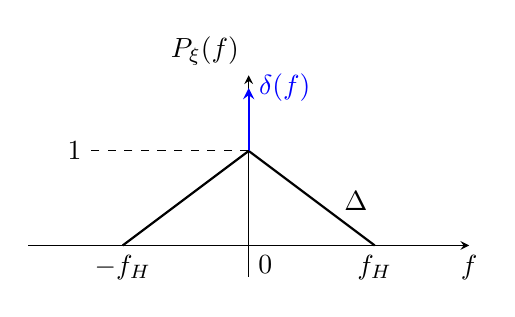
\begin{tikzpicture}[>=stealth, scale=0.8]
                % --- 坐标轴调整 ---
                \draw[->] (-3.5,0) -- (3.5,0) node[below] {$f$};
                % [修改点1]: 将纵轴标签移到左上方,避免与右侧的 delta(f) 标签打架
                \draw[->] (0,-0.5) -- (0,2.7) node[above left] {$P_{\xi}(f)$};
                % --- 三角波 ---
                \draw[thick] (-2,0) -- (0,1.5) -- (2,0);
                % [修改点2]: 将三角符号向右移动 (x坐标从 1.2 改为 1.7)
                \node at (1.7, 0.7) {$\Delta$};
                % --- 直流冲击 delta(f) ---
                % 保持粗线条和蓝色,绘制在坐标轴上方,标签在右侧
                \draw[->, thick, blue] (0,1.5) -- (0,2.5) node[right] {$\delta(f)$};
                % --- 刻度 ---
                \node[below] at (-2,0) {$-f_H$};
                \node[below] at (2,0) {$f_H$};
                \node[below right] at (0,0) {$0$};
                
                % --- 标注峰值 ---
                \draw[dashed] (0,1.5) -- (-2.5, 1.5);
                \node[left] at (-2.5, 1.5) {$1$};
            \end{tikzpicture}
        \end{center}
    
    \tcbline
    
    \textbf{1. 预备知识:傅里叶变换对的推导}
    
    为了求解本题,我们需要建立门函数 $g_{f_H}(f)$ 与抽样函数 $Sa(\cdot)$ 的对应关系。这里提供两种推导方法:
    
    \textbf{方法一:定义法 (积分推导)}
    \begin{itemize}
        \item \textbf{变量对照表}:
        \begin{center}
            \renewcommand{\arraystretch}{1.2}
            \begin{tabular}{|c|c|}
                \hline
                $\omega$ & $2\pi f$ \\
                \hline
                $f$ & $\frac{\omega}{2\pi}$ \\
                \hline
            \end{tabular}
        \end{center}
        \item \textbf{推导}:
        \[
        \begin{aligned}
            \mathcal{F}^{-1}[g_{f_H}(f)] &= \int_{-f_H/2}^{f_H/2} 1 \cdot e^{j2\pi f \tau} df \\
            &= \left[ \frac{e^{j2\pi f \tau}}{j2\pi \tau} \right]_{-f_H/2}^{f_H/2} \\
            &= \frac{e^{j\pi f_H \tau} - e^{-j\pi f_H \tau}}{j2\pi \tau} \\
            &= \frac{\sin(\pi f_H \tau)}{\pi \tau} = f_H Sa(\pi f_H \tau)
        \end{aligned}
        \]
    \end{itemize}

    \textbf{方法二:利用线性性质与尺度变换 (根据手写笔记)}
    \begin{itemize}
        \item \textbf{Step 1: 标准变换对} (门宽为 1)
        \[ g_1(f) \leftrightarrow Sa(\pi \tau) \]
        \item \textbf{Step 2: 频域尺度变换} (引入 $f_H$)
        利用性质 $X(f/k) \leftrightarrow |k|x(k\tau)$。令 $k=f_H$:
        \[ g_{f_H}(f) = g_1\left(\frac{f}{f_H}\right) \leftrightarrow f_H Sa(\pi f_H \tau) \]
        \item \textbf{Step 3: 线性性质/幅度缩放} (构造题目系数)
        题目需构造系数 $A = \frac{1}{\sqrt{f_H}}$。求 $\frac{1}{\sqrt{f_H}} g_{f_H}(f)$ 的逆变换。
        两边同乘 $\frac{1}{\sqrt{f_H}}$:
        \[ \frac{1}{\sqrt{f_H}} g_{f_H}(f) \leftrightarrow \frac{1}{\sqrt{f_H}} \cdot [f_H Sa(\pi f_H \tau)] \]
        化简右边系数 $\frac{f_H}{\sqrt{f_H}} = \sqrt{f_H}$,得最终变换对:
        \[ \boxed{\frac{1}{\sqrt{f_H}} g_{f_H}(f) \leftrightarrow \sqrt{f_H} Sa(\pi f_H \tau)} \]
    \end{itemize}

    \tcbline
    
    \textbf{2. 功率谱密度 $P_\xi(f)$ 的分解与参数求解}
    
    由图可知,$P_\xi(f) = \Delta(f) + \delta(f)$。
    
    \textbf{求解三角形 $\Delta(f)$ 的构成:}
    三角形可视为两个相同门函数 $A \cdot g_{f_H}(f)$ 的卷积。
    \[ \Delta(f) = [A \cdot g_{f_H}(f)] * [A \cdot g_{f_H}(f)] \]
    
    根据卷积几何性质:
    \begin{itemize}
        \item 卷积后高度 = $A^2 \cdot \text{门宽} = A^2 f_H$
    \end{itemize}
    
    由图知三角形顶点高度为 $1$,故 $A^2 f_H = 1 \implies A = \frac{1}{\sqrt{f_H}}$。
    即:
    \[ \Delta(f) = \left[ \frac{1}{\sqrt{f_H}} g_{f_H}(f) \right] * \left[ \frac{1}{\sqrt{f_H}} g_{f_H}(f) \right] \]

    \tcbline
    
    \textbf{3. 求解自相关函数 $R(\tau)$}
    
    利用维纳-辛钦定理及“频域卷积 $\leftrightarrow$ 时域相乘”:
    
    \[
    \begin{aligned}
        R(\tau) &= \mathcal{F}^{-1}[\Delta(f)] + \mathcal{F}^{-1}[\delta(f)] \\
        &= \mathcal{F}^{-1}\left\{ \left[ \frac{1}{\sqrt{f_H}} g_{f_H}(f) \right] * \left[ \frac{1}{\sqrt{f_H}} g_{f_H}(f) \right] \right\} + 1 \\
        &= \left( \mathcal{F}^{-1}\left[ \frac{1}{\sqrt{f_H}} g_{f_H}(f) \right] \right)^2 + 1 
    \end{aligned}
    \]
    代入步骤1中推导出的结论:
    \[
    \begin{aligned}
        R(\tau) &= \left( \sqrt{f_H} Sa(\pi f_H \tau) \right)^2 + 1 \\
        &= f_H Sa^2(\pi f_H \tau) + 1
    \end{aligned}
    \]
    
    \tcbline
    \textbf{4. 功率计算}
    \begin{itemize}
        \item 平均功率 $R(0) = f_H + 1$
        \item 直流功率 $R(\infty) = 1$
        \item 交流功率 $\sigma^2 = f_H$
    \end{itemize}
\end{examplebox}

\end{document}